%%%%%%%%%%%%%%%%%%%%%%%%%%%%%%%%%%%%%%%%%%%%%%%%%%%%%%%%%%%%%%%%%%%%%%%%%%%%%%%%
%%%%%%%%%%%%%%%%%%%%%%%%%%%%%%%%%%%%%%%%%%%%%%%%%%%%%%%%%%%%%%%%%%%%%%%%%%%%%%%%
%
% A general frame for lecture slides and lecture notes in one file
% using LaTeX beamer
%
%%%%%%%%%%%%%%%%%%%%%%%%%%%%%%%%%%%%%%%%%%%%%%%%%%%%%%%%%%%%%%%%%%%%%%%%%%%%%%%%
%%%%%%%%%%%%%%%%%%%%%%%%%%%%%%%%%%%%%%%%%%%%%%%%%%%%%%%%%%%%%%%%%%%%%%%%%%%%%%%%
\documentclass[aspectratio=169,11pt]{beamer}
%\usepackage[ngerman]{babel}
\usepackage[T1]{fontenc}
\usepackage[utf8]{inputenc}
\usepackage{amsmath,amssymb,amsfonts}


% only presentation
\mode<presentation>
{
  \usepackage[course]{dunestyle-beamer}
}

\colorlet{listingbg}{blue!30!black!5!white}
\usepackage[outputdir=@CMAKE_CURRENT_BINARY_DIR@]{minted}

% all after
\usepackage{amscd}

\usepackage{pgfplots,adjustbox}
\usepackage{eurosym}
\usepackage{graphicx}
\graphicspath{{.}{figures/}{../../latexstyle/layout/}}
%\usepackage{picinpar}
%\usepackage{fancybox}
%\usepackage{xspace}
\usepackage{enumerate}
\usepackage{algpseudocode}
\usepackage{color}
\usepackage{bold-extra}
\usepackage{bm}
\usepackage{stmaryrd}
%\usepackage[squaren]{SIunits}
\usepackage{nicefrac}

\usepackage{fancyvrb,bbm,xspace}
\usepackage{lmodern}
\usepackage{fancyvrb,bbm,xspace}
\usepackage[binary-units]{siunitx}
\usepackage{xcolor,tabu}
\usepackage{booktabs}

\usepackage{lmodern}
\usepackage{inconsolata}
\usepackage{nimbusmononarrow}
%\renewcommand*\ttdefault{txtt}
\usepackage{dsfont}

\mode<presentation>
{
\theoremstyle{definition}
}
\newtheorem{Def}{Definition}%[section]
\newtheorem{Exm}[Def]{Example}
\newtheorem{Lem}[Def]{Lemma}
\newtheorem{Rem}[Def]{Remark}
\newtheorem{Rul}[Def]{Rule}
\newtheorem{Thm}[Def]{Theorem}
\newtheorem{Cor}[Def]{Corollary}
\newtheorem{Obs}[Def]{Observation}
\newtheorem{Ass}[Def]{Assumption}
\newtheorem{Pro}[Def]{Property}
\newtheorem{Alg}[Def]{Algorithm}
\newtheorem{Prp}[Def]{Proposition}
\newtheorem{Lst}[Def]{Listing}


%% Typesetting C++
\def\CC{{C\nolinebreak[4]\hspace{-.05em}\raisebox{.4ex}{\tiny\bf ++}}}

% Delete this, if you do not want the table of contents to pop up at
% the beginning of each subsection:
\AtBeginSection[]
{
  \begin{frame}<beamer>
    \frametitle{Contents}
    \tableofcontents[sectionstyle=show/shaded,subsectionstyle=hide/hide/hide]
%\tableofcontents[currentsection]
  \end{frame}
}

% Title definition
\title{DUNE PDELab Tutorial 09}
\subtitle{Using Code Generation to Create Local Operators}
\author{PDELab Team}
\institute[]
{
  IWR\\
  Heidelberg University
}

%%%%%%%%%%%%%%%%%%%%%%%%%%%%%%%%%%%%%%%%%%%%%%%%%%%%%%%%%%%%%%%%%%%%%%%%%%%%%%%%
%%%%%%%%%%%%%%%%%%%%%%%%%%%%%%%%%%%%%%%%%%%%%%%%%%%%%%%%%%%%%%%%%%%%%%%%%%%%%%%%
%
% now comes the individual stuff lecture by lecture
%
%%%%%%%%%%%%%%%%%%%%%%%%%%%%%%%%%%%%%%%%%%%%%%%%%%%%%%%%%%%%%%%%%%%%%%%%%%%%%%%%
%%%%%%%%%%%%%%%%%%%%%%%%%%%%%%%%%%%%%%%%%%%%%%%%%%%%%%%%%%%%%%%%%%%%%%%%%%%%%%%%

\begin{document}

\frame[plain, noframenumbering]{\titlepage}

%%%%%%%%%%%%%%%%%%%%%%%%%%%%%%%%%%%%%%%%%%%%%%%%%%%%%%%%%%%%%%%%%%%%%%%%%%%%%%%%
%%%%%%%%%%%%%%%%%%%%%%%%%%%%%%%%%%%%%%%%%%%%%%%%%%%%%%%%%%%%%%%%%%%%%%%%%%%%%%%%
\section{Introduction}

\begin{frame}[fragile]
  \frametitle{Introduction}
  \textbf{Introduction}
  \begin{itemize}
  \item This tutorial gives a short introduction to using
    \lstinline{dune-codegen}\footnote{https://gitlab.dune-project.org/extensions/dune-codegen}
  \item \lstinline{dune-codegen} uses code generation to solve PDEs. This is
    done by describing the PDE in a domain-specific language (DSL) and
    generating \CC\ code for the local integration kernels
  \item We use UFL\footnote{https://bitbucket.org/fenics-project/ufl} as DSL
  \item The generated code can be used in \lstinline{dune-pdelab}
  \item This makes it easier to use PDELab for your application
  \end{itemize}
\end{frame}

\begin{frame}
  \frametitle{Introduction}
  We will look at a quick example to get some idea how this looks like.
\end{frame}

\begin{frame}
  \frametitle{Hello World: Poisson Problem}

  \begin{itemize}
  \item Strong formulation:
    \begin{align*}
      -\Delta u & = f \qquad\text{in $\Omega$}, \\
      u &= g \qquad\text{on $\partial\Omega$},
    \end{align*}
  \item Discrete weak formulation: Find $u_h \in U_h$ with
    \begin{equation*}
      r_h^{Poisson}(u_h, v_h) = \int_\Omega \nabla u_h \cdot \nabla v_h \, dx
      - \int_\Omega f \, v_h \, dx = 0 \qquad \forall v_h \in V_h
    \end{equation*}
  \item Parameter functions:
    \begin{align*}
      f(x) = -2d \\
      g(x) = \| x \|_2^2
    \end{align*}
  \end{itemize}
\end{frame}

\begin{frame}
  \frametitle{UFL file for Poisson Problem}

  Discrete weak formulation: Find $u_h \in U_h$ with
  \begin{equation*}
    r_h^{Poisson}(u_h, v_h) = \int_\Omega \nabla u_h \cdot \nabla v_h \, dx
    - \int_\Omega f \, v_h \, dx = 0 \qquad \forall v_h \in V_h
  \end{equation*}
  \lstinputlisting[basicstyle=\scriptsize, backgroundcolor=\color{listingbg}]{../src/poisson.ufl}
\end{frame}

\begin{frame}
  \frametitle{Goals of this Talk}

  \textbf{Goals of this talk}
  \begin{itemize}
  \item Explain how to write down PDEs in UFL
  \item Show how \lstinline{dune-codegen} modifies/extends UFL
  \item Show how it is integrated into the build system
  \end{itemize}
  \vfill
  \textbf{Before this we will}
  \begin{itemize}
  \item Give a short overview over the workflow
  \item Talk about differences to other code generation approaches
  \end{itemize}
\end{frame}

\begin{frame}
  \frametitle{Resources}
  This tutorial is partially based on
  \begin{itemize}
  \item ``Code Generation for High Performance PDE Solvers
    on Modern Architectures'' by Dominic Kempf
  \item ``Unified Form Language: A domain-specific language for weak
    formulations of partial differential equations'' M. S. Alnaes, A. Logg,
    K. B. Ølgaard, M. E. Rognes and G. N. Wells
  \item UFL documentation
    \url{https://fenics.readthedocs.io/projects/ufl/en/latest/index.html}
  \end{itemize}

\end{frame}
\section{The Big Picture}

\begin{frame}[fragile]
  \frametitle{The Big Picture}
  \begin{itemize}
  \item Research goals of \lstinline{dune-codegen}:
    \begin{itemize}
    \item Generate high performance code
    \item Do performance optimizations on intermediate representation (in our
      case Loopy\footnote{https://mathema.tician.de/software/loopy/}),
      e.g. SIMD vectorization
    \end{itemize}
  \item Difference to other code generation approaches:
    \begin{itemize}
    \item Do not generate everything. Instead generate code against a well
      defined interface of a \CC\ framework.
    \item The workflow is CMake and \CC\ driven and not controlled through
      Python.
    \item Main focus on generating high performance code
    \end{itemize}
  \end{itemize}
\end{frame}

\begin{frame}
  \frametitle{Typical Workflow}
  \begin{itemize}
  \item Have a dune module that depends on \lstinline{dune-codegen}
  \item Write a UFL file describing the PDE
  \item Add a target in CMake (see build system part)
  \item Go to the build directory and type make. CMake will generate the \CC\
    code and compile the executable.
  \end{itemize}
\end{frame}

\begin{frame}
 \frametitle{Form Compiler Approach}
 \centering
 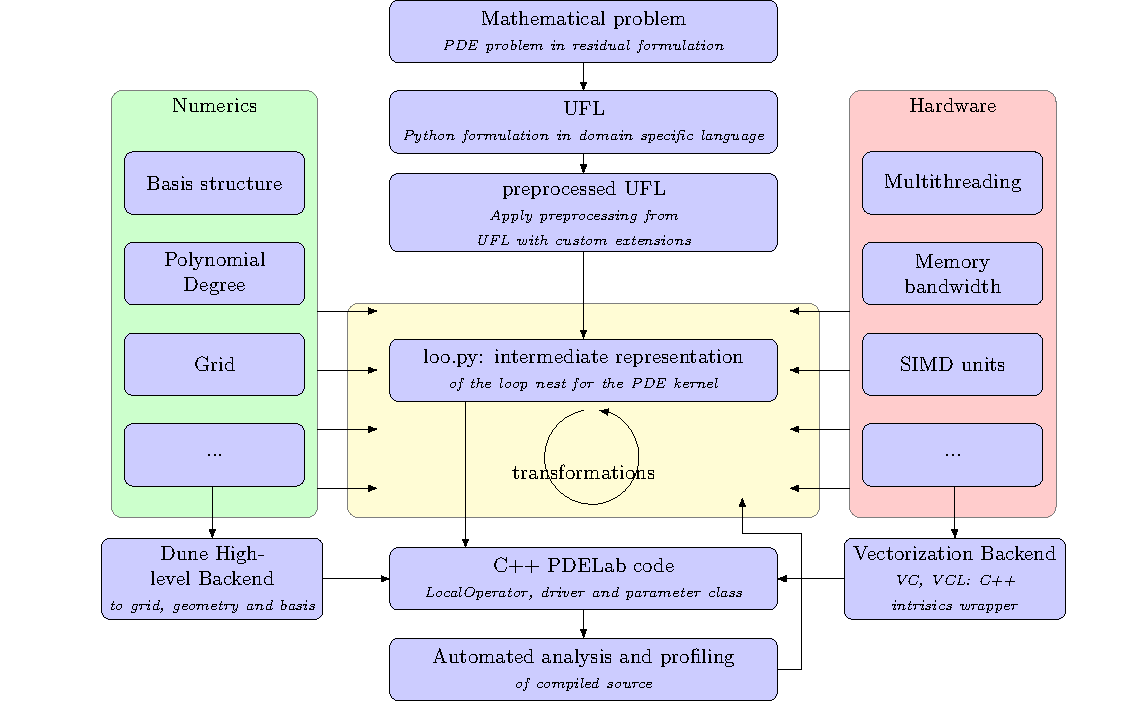
\includegraphics[width=4.5in]{./figures/approach.pdf}
\end{frame}


\section{Hello World: Poisson}

\begin{frame}
  \frametitle{UFL: Poisson}
  Discrete weak formulation: Find $u_h \in U_h$ with
  \begin{equation*}
    r_h^{Poisson}(u_h, v_h) = \int_\Omega \nabla u_h \cdot \nabla v_h \, dx
    - \int_\Omega f \, v_h \, dx = 0 \qquad \forall v_h \in V_h
  \end{equation*}

  UFL file:
  \lstinputlisting[basicstyle=\scriptsize, backgroundcolor=\color{listingbg},
]{../src/poisson.ufl}
\end{frame}

\begin{frame}
  \frametitle{UFL: About}
  \begin{itemize}
  \item Domain specific language for describing weak formulations of PDE
    discretizations
  \item Notation stays close to methematical formulation
  \item Embedded in Python
  \item Only desribes cell/facet local computations. There is no notion of a
    grid or a description of an element loop
  \item The form is described by an abstract syntax trees (AST)
  \item UFL can apply transformation on the AST e.g.:
    \begin{itemize}
    \item Calculation of the Jacobian of the residual
    \item Geometry lowering
    \end{itemize}
  \end{itemize}
\end{frame}

\begin{frame}
  \frametitle{UFL: AST}
  \centering
  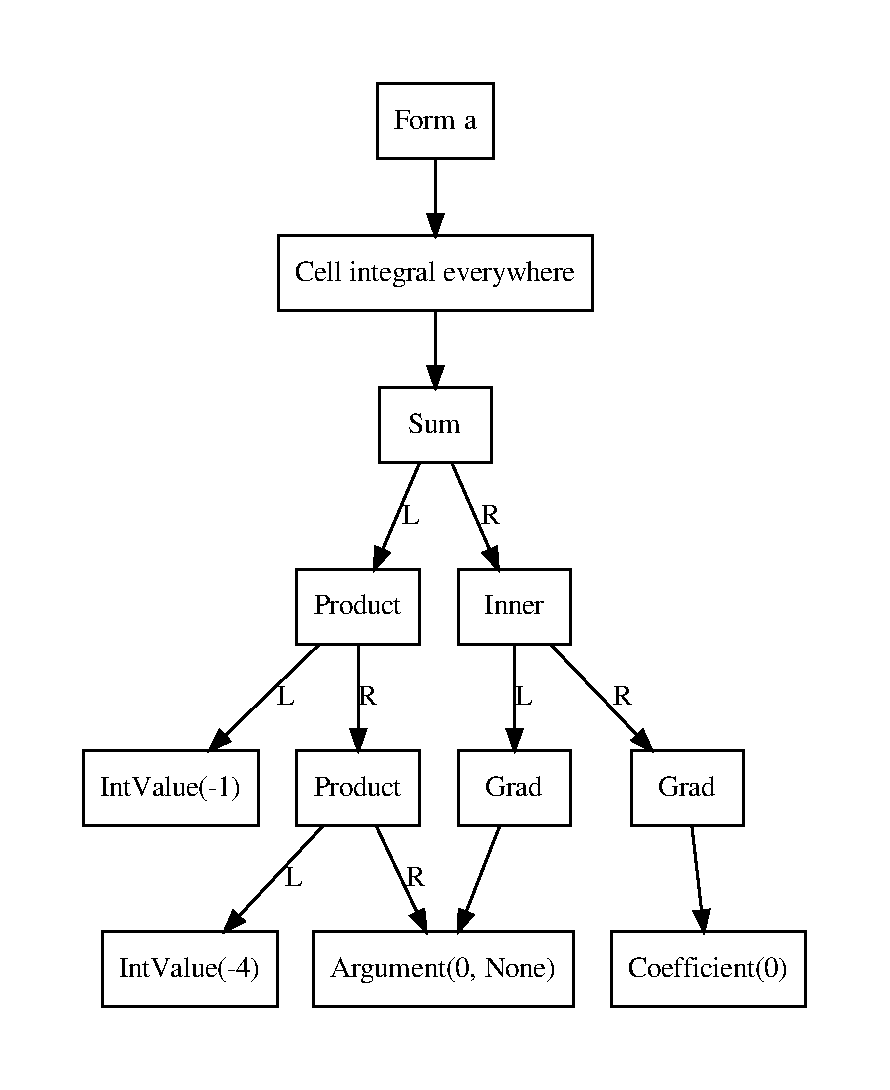
\includegraphics[scale=0.4]{figures/ufl_ast.pdf}
\end{frame}

\begin{frame}
  \frametitle{UFL: AST - Preprocessed}
  \centering
  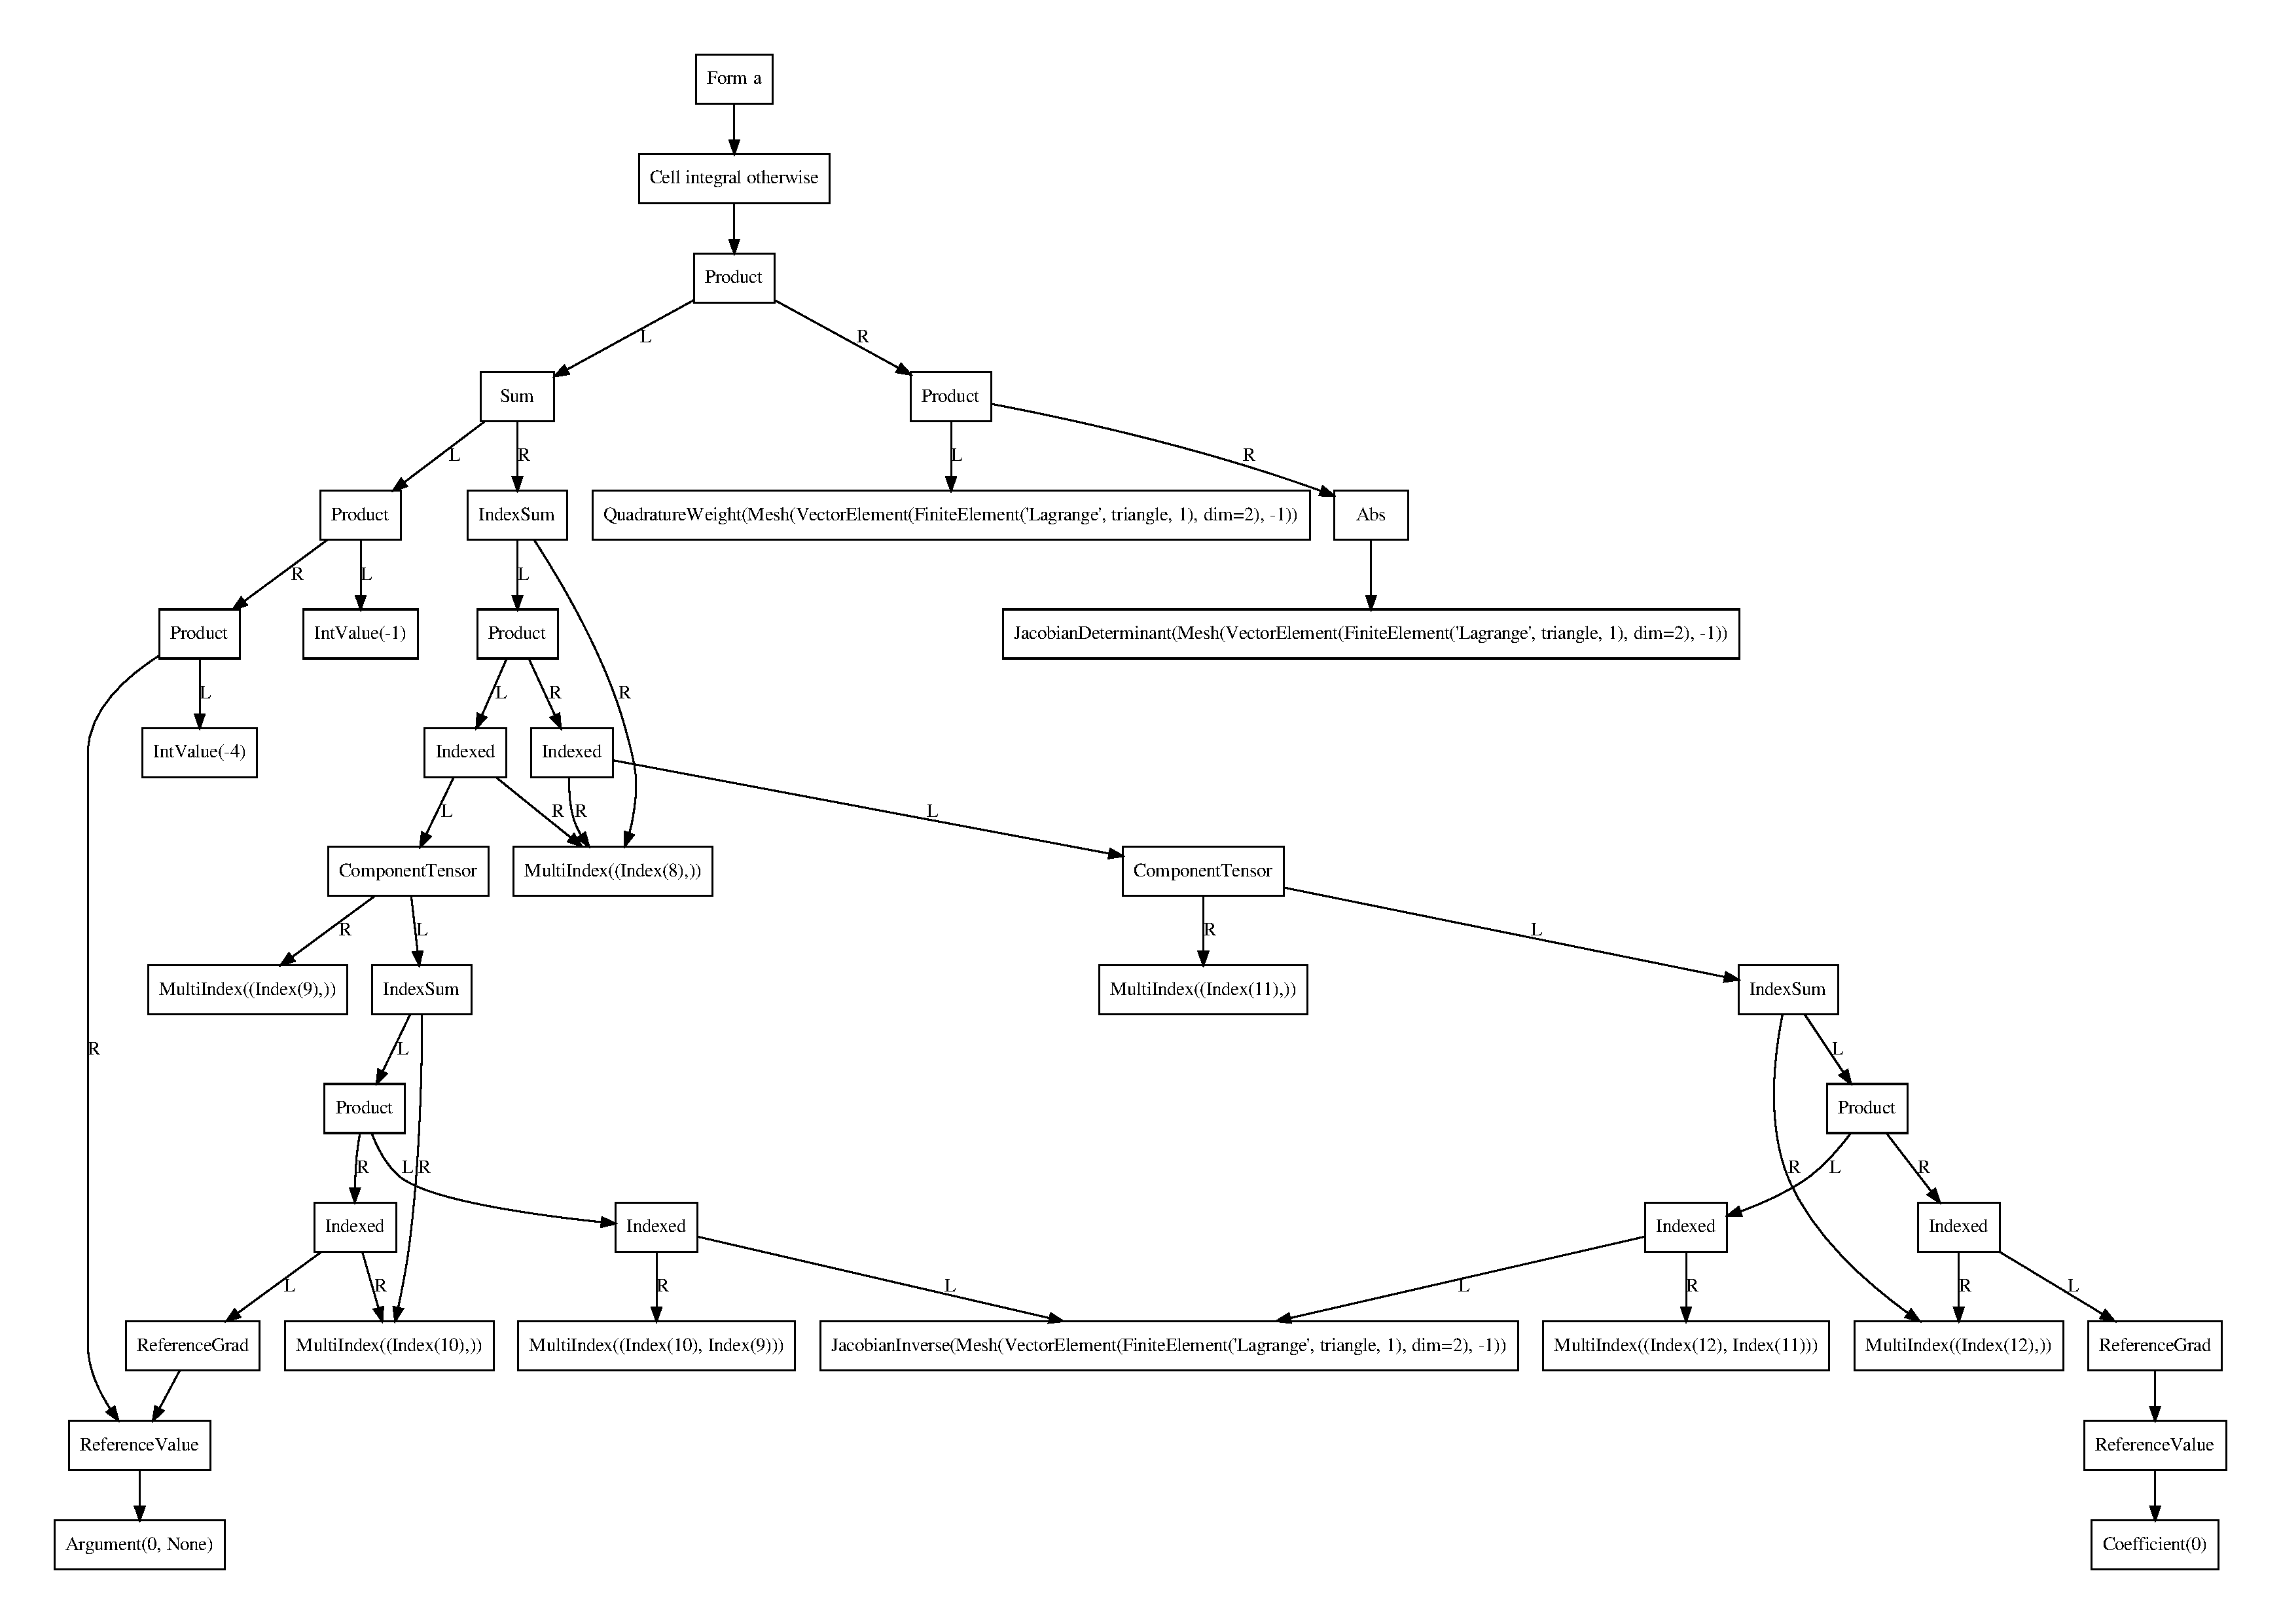
\includegraphics[scale=0.2]{figures/ufl_ast_preprocessed.pdf}
\end{frame}

\begin{frame}[fragile]
  \frametitle{UFL: \lstinline{FiniteElement}}
  \begin{lstlisting}
V = FiniteElement(family, cell, degree)
  \end{lstlisting}
  \vfill
  \begin{itemize}
  \item family: String representing a finite element family
    \begin{itemize}
    \item \lstinline{'CG'} Continuous Lagrange finite element
    \item \lstinline{'DG'} Discontinuous Galerkin Lagrange finite element
    \end{itemize}
  \item Possible Cells:
    \begin{tabu}{ccc}
      Dimension & Simplex Cell & Cube Cell \\
      $0$ & \lstinline{vertex} & \lstinline{vertex} \\
      $1$ & \lstinline{interval} & \lstinline{interval} \\
      $2$ & \lstinline{triangle} & \lstinline{quadrilateral} \\
      $3$ & \lstinline{tetrahedron} & \lstinline{hexahedron} \\
    \end{tabu}
  \item Instead you can also write \lstinline{Cell('triangle')}
  \item \lstinline{degree}: Polynomial degree
  \end{itemize}
\end{frame}

\begin{frame}
  \frametitle{UFL: Form}
  \begin{itemize}
  \item UFL expresses forms
    \begin{align*}
      a: W_1\times\dots\times W_m\times V_1\times\dots\times V_n & \rightarrow \mathbb{R} \\
      (w_1,\dots ,w_m,v_1,\dots ,v_n) & \mapsto a(w_1,\dots ,w_m;v_1,\dots ,v_n)
    \end{align*}
  \item Linear in the arguments $v_1,\dots,v_n$
  \item Possibly nonlinear in coefficient functions $w_1,\dots,w_m$
  \item PDELab uses a residual formulation: Find $u\in U$ with
    \begin{align*}
      r(u,v) = 0 \qquad \forall v \in V
    \end{align*}
  \item $r$ is linear in $v$ but might be nonlinear in $u$
  \end{itemize}
\end{frame}

\begin{frame}[fragile]
  \frametitle{UFL: \lstinline{TrialFunction} and \lstinline{TestFunction}}

  \lstinputlisting[basicstyle=\scriptsize, backgroundcolor=\color{listingbg}, linerange={3-4}]{../src/poisson.ufl}
  \vfill
  \begin{itemize}
  \item \lstinline{TrialFunction} and \lstinline{TestFunction} represent finite element functions.
  \item Take \lstinline{FiniteElement} as argument
  \item Note: In contrast to other UFL based frameworks our forms need not be
    linear in the \lstinline{TrialFunction}
  \end{itemize}
\end{frame}

\begin{frame}
  \frametitle{UFL: Defining Expressions}
  \lstinputlisting[basicstyle=\scriptsize, backgroundcolor=\color{listingbg}, linerange={6-11}]{../src/poisson.ufl}
  \vfill
  \begin{itemize}
  \item \lstinline{SpatialCoordinate}: Global coordinate
  \item \lstinline{grad(u)}: Gradient of $u$
  \item \lstinline{inner(A,B)}: Inner product
    \begin{equation*}
      A:B = \sum_{i_0}\cdots\sum_{i_{n-1}}A_{i_0\cdots i_{n-1}}B_{i_0\cdots i_{n-1}}
    \end{equation*}
  \item \lstinline{dx}: Multiplication with \lstinline{dx} indicates a volume
    integral
  \end{itemize}
\end{frame}

\begin{frame}
  \frametitle{UFL: \lstinline{dune-codegen} Specific}
  \lstinputlisting[basicstyle=\scriptsize, backgroundcolor=\color{listingbg}, linerange={13-16}]{../src/poisson.ufl}
  \vfill
  \begin{itemize}
  \item Main goal of \lstinline{dune-codegen} is to generate the local integration kernel
  \item For testing and solving simple problem an automated driver can be
    generated. For the correct handling of the boundary condition we need to
    add some information to the UFL file
  \item \lstinline{exact_solution}: Can be set for writing tests if solution is known
  \item \lstinline{is_dirichlet}: Expression that may depend on $x$ and returns
    $1$ if this is a dirichlet boundary condition. This is used only for driver
    generation.
  \item \lstinline{interpolate_expression}: This is used as Dirichlet boundary value
  \item \lstinline{dune-codegen} imports everything from the UFL module via
    \lstinline{from UFL import *}
  \end{itemize}
\end{frame}

\section{UFL: Towards More Complex Forms}

\begin{frame}
  \frametitle{UFL: Towards More Complex Forms}
  In the following we show some important features of UFL. This is by no means
  complete, see the official documentation for further details
  \url{https://fenics.readthedocs.io/projects/ufl/en/latest/index.html}.
\end{frame}

\begin{frame}[fragile]
  \frametitle{UFL: Math Expressions}
  \begin{itemize}
  \item Math functions, e.g. \lstinline{*}, \lstinline{/}, \lstinline{+},
    \lstinline{-}, \lstinline{abs}, \lstinline{exp}, \lstinline{ln},
    \lstinline{sqrt}, trigonometric functions, ...
  \item Comparison operator: \lstinline{eq}, \lstinline{ne}, \lstinline{le},
    \lstinline{ge}, \lstinline{lt} and \lstinline{gt}
  \item Conditionals:
    \begin{displaymath}
      \text{\lstinline{conditional(cond, A, B)}} = \left\{
        \begin{array}{lr}
          \text{\lstinline{A}}\ \ \ \ & \text{\lstinline{cond is True}} \\
          \text{\lstinline{B}} & \text{\lstinline{cond is False}}
        \end{array}
      \right.
    \end{displaymath}
  \item Vector-, matrix- and tensor-valued objects can be created through
    \lstinline{as_vector}, \lstinline{as_matrix} and \lstinline{as_tensor}
    \begin{lstlisting}
a = as_matrix([[1.0, 2.0],[3.0, 4.0]])
    \end{lstlisting}
  \item See the official documentation for tensor algebra operations
  \end{itemize}
\end{frame}

\begin{frame}[fragile]
  \frametitle{UFL: Geometric Quantities}
  \begin{itemize}
  \item \lstinline{SpatialCoordinate(cell)}: Global coordinate
  \item \lstinline{FacetNormal(cell)}: Unit outer normal vector
  \item \lstinline{CellVolume(cell)} and   \lstinline{FacetArea(cell)}
  \end{itemize}
\end{frame}

\begin{frame}[fragile]
  \frametitle{UFL: Integral Measures}
  \begin{itemize}
  \item Multiplication with a measure describes an integral object over a local
    cell or facet
  \item \lstinline{dx}: Integral over cell
  \item \lstinline{ds}: Integral over boundary facet
  \item \lstinline{dS}: Integral over interior facet
  \item Measures can be restricted to a subdomain. See the example about mixed
    Dirichlet and Neumann conditions on the next slides
  \end{itemize}
\end{frame}

\begin{frame}
  \frametitle{Example: Mixed Boundary Conditions}

  Strong formulation:
  \begin{align*}
    -\Delta u + q(u) & = f \qquad\text{in $\Omega$}, \\
    u &= g \qquad\text{on $\Gamma_D\subset\partial\Omega$}, \\
    -\nabla u \cdot \nu &= j \qquad\text{on $\Gamma_N\subset\partial\Omega$}
  \end{align*}

  Weak discrete formulation: Find $u_h \in U_h$ with
  \begin{align*}
    r_h^{NLP}(u_h, v_h)
    & = \int_\Omega \nabla u_h \cdot \nabla v_h \, dx
      + \int_\Omega q(u) \, v \, dx \\
    &\quad - \int_\Omega f \, v_h \, dx
      + \int_{\Gamma_N} j \, v \, ds
      = 0 \qquad \forall v_h \in V_h
  \end{align*}

  Parameter functions:
  \begin{align*}
    f(x) = -2d \\
    g(x) = \| x \|_2^2\\
    j(x) = -
    \begin{pmatrix}
      2x_0 \\ 2x_1
    \end{pmatrix}
    \cdot \nu
  \end{align*}
\end{frame}

\begin{frame}
  \frametitle{Example: Mixed Boundary Conditions}
  \lstinputlisting[basicstyle=\tiny,  backgroundcolor=\color{listingbg}]{../src/nonlinear_poisson.ufl}
\end{frame}

\begin{frame}[fragile]
  \frametitle{UFL: DG Operators} UFL provides operators for implementation of
  Discontinuous Galerkin (DG) methods. These methods are discontinuous at
  interior facets. This means you have two values for the 'inside' cell and the
  'outside' cell.
  \begin{itemize}
  \item \lstinline{avg(u)}: Average between those values
    $\frac{1}{2}(u|_{T^+}+u|_{T^-})$
  \item \lstinline{jump(u)}: Difference between the values $u|_{T^+}-u|_{T^-}$
  \item Restriction: Expression can be restricted to the inside or the outside
    cell by typing \lstinline{u('+')} or \lstinline{u('-')}\footnote{In the
      literature '-' usually denotes the inside and '+' the outside cell.}
  \end{itemize}
\end{frame}

\begin{frame}[fragile]
  \frametitle{UFL: FiniteElement}
  \textbf{VectorElement}\\
  \lstinline[basicstyle=\small]{V= VectorElement(family, cell, degree[, size])}
  \begin{itemize}
  \item Combination of a basic element for a vector field
  \item \lstinline{familty}, lstinline{cell}, \lstinline{degree} like \lstinline{FiniteElement} above
  \item \lstinline{size}: Optional, default equal to dimension
  \end{itemize}

  \textbf{TensorElement}\\
  \lstinline[basicstyle=\small]{V = TensorElement(family, cell, degree[, shape, symmetry])}
  \begin{itemize}
  \item Like \lstinline{VectorElement} but for \lstinline{shape} given as tuple
  \item Symmetry can be expressed as Python dictionary
    \lstinline|symmetry={(0,1): (1,0)}|
  \end{itemize}


  \textbf{MixedElement}\\
  \lstinline[basicstyle=\small]{V = MixedElement(element1, element2[,...])}
  \begin{itemize}
  \item Arbitrary combination of finite elements
  \item Can also be created like this \lstinline{V = element1*element2}
  \end{itemize}
\end{frame}


\begin{frame}[fragile]
  \frametitle{UFL: Trialfunctions and Testfunctions}
  \begin{itemize}
  \item You can get the test- and trialfunctions of these spaces using the
    \lstinline{split} command
  \begin{lstlisting}[basicstyle=\small, backgroundcolor=\color{listingbg}]
FE_V = VectorElement('CG', triangle, 2)
FE_P = FiniteElement('CG', triangle, 1)
TH = FE_V * FE_P
u, p = split(TrialFunction(TH))
v, q = split(TestFunction(TH))
  \end{lstlisting}
  \item There is also an abbreviation (don't miss the additional s)
    \begin{lstlisting}[basicstyle=\small, backgroundcolor=\color{listingbg}]
u, p = TrialFunctions(TH)
v, q = TestFunctions(TH)
    \end{lstlisting}
  \end{itemize}
  % TODO: Maybe write something about u=Trialfunction(V) und u[0] and u[1] but
  % I'm not sure how that works out for Navier Stokes ;)
\end{frame}

\begin{frame}
  \frametitle{Example: Wave Equation as First Order System}
  Strong formulation as first order system:
  \begin{subequations}
    \label{eq:SystemForm1}
    \begin{align*}
      \partial_t u_1 - c^2\Delta u_0 &=0 &&\text{in $\Omega\times\Sigma$},\\
      \partial_t u_0 - u_1 &=0 &&\text{in $\Omega\times\Sigma$},\\
      u_0 &= 0 &&\text{on $\partial\Omega$},\\
      u_1 &= 0 &&\text{on $\partial\Omega$},\\
      u_0 &= q &&\text{at $t=0$},\\
      u_1 &= w &&\text{at $t=0$}.
    \end{align*}
  \end{subequations}

  Weak discrete formulation: Find $(u_0(t),u_1(t))\in U_0\times U_1$ s.t.
  \begin{align*}
    d_t (u_1,v_0)_{0,\Omega} + c^2 (\nabla u_0, \nabla v_0)_{0,\Omega}
    &= 0 \quad \forall v_0 \in U_0 \notag \\
    d_t (u_0,v_1)_{0,\Omega} - (u_1,v_1)_{0,\Omega}
    &= 0 \quad \forall v_1 \in U_1
  \end{align*}

  Parameters: Speed of sound $c=1$
\end{frame}

\begin{frame}[fragile]
  \frametitle{Example: Wave Equation as First Order System}

  \begin{align*}
    d_t (u_1,v_0)_{0,\Omega} + c^2 (\nabla u_0, \nabla v_0)_{0,\Omega}
    &= 0 \quad \forall v_0 \in U_0 \notag \\
    d_t (u_0,v_1)_{0,\Omega} - (u_1,v_1)_{0,\Omega}
    &= 0 \quad \forall v_1 \in U_1
  \end{align*}

  \lstinputlisting[basicstyle=\scriptsize, lastline=14, backgroundcolor=\color{listingbg}]{../src/wave_equation.ufl}
\end{frame}

\begin{frame}[fragile]
  \frametitle{UFL: Derivatives}
  \begin{itemize}
  \item \lstinline{grad(u)}: Gradient of u
  \item \lstinline{div(u)}: Divergence of u
  \item \lstinline{curl(u)}: Curl of u (only for finite element functions with
    three components)
  \item \lstinline{u.dx(d)}: D'th partial derivative $\frac{\partial u}{\partial x_d}$
  \item UFL can also compute derivatives of forms or expressions wrt to
    \lstinline{Variables} or \lstinline{Coefficients} (Note: In
    \lstinline{dune-codegen} the \lstinline{TrialFunction} is a
    \lstinline{Coefficient})
    \begin{lstlisting}[basicstyle=\scriptsize, backgroundcolor=\color{listingbg}]
u = Coefficient(element)
w = sin(u**2)
w = variable(w)
F = w**2

# Derivative of expression F
dF_w = diff(F, w)
dF_u = diff(F, u)
    \end{lstlisting}
  \end{itemize}
\end{frame}

\begin{frame}[fragile]
  \frametitle{UFL: \lstinline{dune-codegen} Specific}
  \begin{itemize}
  \item As mentioned before \lstinline{dune-codegen} uses the residual
    formulation. The provided residual form may be nonlinear in the trial
    function.\footnote{In our case the trialfunction is a Coefficient and not
      an Argument.}
  \item Your UFL file may contain multiple forms. \lstinline{dune-codegen} will
    generate local operators for all forms listed in the ini file, eg
    \inputminted[fontsize=\small, firstline=12, lastline=13]{ini}{../src/heatequation.ini}
  \item See the build system part of this tutorial for more options!
  \end{itemize}
\end{frame}

\begin{frame}[fragile]
  \frametitle{UFL: \lstinline{dune-codegen} Specific}
  \begin{itemize}
  \item For testing automated drivers can be generated. We use the following
    convention for instationary problems: If there are exactly two forms and
    one is called \lstinline{mass} we assume that the problem is instationary
    and generate a suitable driver.\footnote{Keep in mind that
      \lstinline{dune-codegen} was developed to generate local operator. The
      driver generation was mainly done for testing.}
  \item Instationary problems can have time dependent parameters but UFL has no
    notion of time. In \lstinline{dune-codegen} you can get a variable
    representing the time by
    \begin{lstlisting}[basicstyle=\scriptsize, backgroundcolor=\color{listingbg}]
t = get_time(cell)
    \end{lstlisting}
    \end{itemize}
\end{frame}

\begin{frame}
  \frametitle{Example: Heatequation}
  \lstinputlisting[basicstyle=\tiny, backgroundcolor=\color{listingbg}]{heatequation_gen.ufl}
\end{frame}


\section{Build System Integration}

\begin{frame}[fragile]
  \frametitle{CMake: \lstinline{dune_add_generated_executable}}

  \begin{itemize}
  \item We need to generate \CC\ code and compile it
  \item Add a code generation target to your \lstinline{CMakeLists.txt}
    \inputminted[fontsize=\scriptsize]{cmake}{generated_executable.txt}
  \item \lstinline{UFLFILE}: UFL file describing the PDE
  \item \lstinline{INIFILE}: Ini file with code generation option under \lstinline{[formcompiler]} section
  \item \lstinline{TARGET}: Name of the executable
  \item \lstinline{SOURCE}: \CC\ file used for building the target. This is
    optional, if omitted a minimal driver willl be generated
  \end{itemize}
\end{frame}

\begin{frame}[fragile]
  \frametitle{CMake: \lstinline{dune_add_generated_executable}}

  \begin{itemize}
  \item Automated driver generation is mainly developed for automated software
    tests
  \item For complicated applications handwritten drivers will be
    necessary. This requires control over the file- and classname of the
    generated local operator.
  \item Can be done in the ini file \vspace{0.3cm}
    \inputminted[fontsize=\scriptsize]{ini}{classname_filename.ini}
  \end{itemize}
\end{frame}

\begin{frame}[fragile]
  \frametitle{Ini File: Global Options}

  \begin{itemize}
  \item \lstinline{operators}: Comma separated list of form names for which
    want to generate operators \lstinline{[default r]}
  \item \lstinline{explicit_time_stepping}: Use explicit time stepping (in
    instationary case) \lstinline{[0/1, default 0]}
  \end{itemize}
\end{frame}

\begin{frame}[fragile]
  \frametitle{Ini File: Form Options}

  \begin{itemize}
  \item Options for a form called \lstinline{r} need to be put into the
    \lstinline{[formcompiler.r]} section
  \item \lstinline{filename}: Name of the generated local
    operator file \lstinline{[str, optional]}
  \item \lstinline{classname}: Name of the local operator class
    \lstinline{[str, optional]}
  \item \lstinline{numerical_jacobian}: Use numerical differentiation for
    assembling the Jacobian of the residual \lstinline{[0/1, default 0]}
  \item \lstinline{quadrature_order}: Order of quadrature \lstinline{[int>0,],optional, guessed by UFL if omitted)}
  \item \lstinline{geometry_mixins}: Information about grid properties that can
    lead to simplified gemometry evaluations
    \lstinline{[generic/axiparallel/equidistant]}
  \end{itemize}
\end{frame}

\begin{frame}[fragile]
  \frametitle{Ini File: Options for Generated Driver}
  \textbf{Grid generation}


  \begin{itemize}
  \item Grid generation options are at the top under no section
  \item Quadrilateral grid
    \inputminted[fontsize=\tiny, firstline=1, lastline=2]{ini}{../src/heatequation.ini}
  \item Simplex grid
    \inputminted[fontsize=\tiny, firstline=1, lastline=4]{ini}{../src/poisson.ini}
  \item Gmsh grid
    \inputminted[fontsize=\tiny, firstline=1, lastline=1]{ini}{../exercise/task/navier_stokes.ini}

  \end{itemize}

\end{frame}

\begin{frame}[fragile]
  \frametitle{Ini File: Options for Generated Driver}
  \vfill
  \textbf{Name of vtk output}
  \begin{itemize}
  \item Under section \lstinline{[wrapper.vtkcompare]}
  \item \lstinline{name}: Basename (without ending) of vtk output
  \end{itemize}
  \vfill
  \textbf{Parameters for Instationary problems}
  \begin{itemize}
  \item Need to be put into the \lstinline{[instat]} section
  \item \lstinline{T}: End of time intervall
  \item \lstinline{dt}: Time step size
  % \item \lstinline{theta}: The one step theta method is used if an implicit
  %   time stepping method of first order is chosen. This is the parameter of the
  %   method
  \item \lstinline{output_every_nth}: Write visualization output for every nth time
    step
  \end{itemize}
  \vfill
\end{frame}

\begin{frame}[fragile]
  \frametitle{CMake: Example Heatequation}

  \lstinputlisting[basicstyle=\tiny, backgroundcolor=\color{listingbg}]{../src/heatequation.ufl}
  \lstinline{CMakeLists.txt}
  \inputminted[fontsize=\tiny, firstline=3, lastline=9]{cmake}{../src/CMakeLists.txt}
\end{frame}

\begin{frame}
  \frametitle{CMake: Example Heatequation}
  \lstinline{heatequation.ini}
  \inputminted[fontsize=\tiny]{ini}{../src/heatequation.ini}
\end{frame}

\begin{frame}[fragile]
  \frametitle{Examples}
  In the folder \lstinline{tutorial09/src} you can find several examples:
  \begin{itemize}
  \item Poisson equation from tutorial00
  \item Nonlinear Poisson equation with mixed boundary from tutorial01
  \item Heat equation from tutorial03
  \item Wave equation from tutorial04
  \end{itemize}

  In the exercises you will additionally find examples for:
  \begin{itemize}
  \item Navier Stokes equation modeling the flow around a cylinder from tutorial08
  \item Discontinuous Galerkin discretization of the Poisson equation
  \end{itemize}
\end{frame}

\end{document}
